%\documentclass[a4paper]{article}
\documentclass{beamer}

\makeatletter
\renewcommand \theequation {%
	\ifnum \c@section>\z@ \@arabic\c@section.\fi \ifnum \c@subsection>\z@
	\@arabic\c@subsection.\fi\ifnum \c@subsubsection>\z@
	\@arabic\c@subsubsection.\fi\@arabic\c@equation}
\@addtoreset{equation}{section}
\@addtoreset{equation}{subsection}
\makeatother
\setcounter{section}{-1}

\setbeamertemplate{caption}[numbered]

\renewcommand\thefigure{\thesection.\thesubsection.\arabic{figure}}
\makeatletter
\@addtoreset{figure}{section}
\@addtoreset{figure}{subsection}
\makeatother

\allowdisplaybreaks

%\usepackage[dvipsnames,table,xcdraw]{xcolor}
%\usepackage{beamerarticle}
\usetheme{Berlin}
%\usetheme{Boadilla}
%\usetheme{Hannover}
\useoutertheme[height=1.5cm]{sidebar}
\usecolortheme{spruce}
\usecolortheme{lily}
\usefonttheme{professionalfonts}
\usepackage{fontspec}
%\usepackage{ctex}
\usepackage{xeCJK}
\usepackage{caption}

\setCJKmainfont{KaiTi}
\setmainfont{Times New Roman}

\usepackage{graphicx}
\usepackage{animate}
\usepackage{amsmath}
%\usepackage{enumitem}
\usepackage{algorithm}
\usepackage{algorithmicx}
\usepackage{algpseudocode}
%\floatname{algorithm}{算法}
\renewcommand{\algorithmicrequire}{\textbf{输入:}}  
\renewcommand{\algorithmicensure}{\textbf{输出:}} 

\usepackage[backend=bibtex,sorting=none]{biblatex}
\addbibresource{cite.bib} %BibTeX数据文件及位置
\setbeamerfont{footnote}{size=\tiny}

\title{图像分割相关算法展示}
\author{\href{mailto:luoyt14thu@gmail.com}{罗雁天}}
\date{\today}
\logo{
\includegraphics[height=1.5cm]{images/Tsinghua2.png}}
%\hyperlinkdocumentend{\logo{
\includegraphics[height=1.5cm]{images/Tsinghua2.png}}}

\newcommand{\upcite}[1]{\textsuperscript{\textsuperscript{\cite{#1}}}}
\setbeamertemplate{bibliography item}[text]
\begin{document}
\begin{frame}{多媒体通信技术}
\titlepage
\end{frame}

\section*{目录}
\begin{frame}{目录}
\tableofcontents
\end{frame}

\section{Introduction}
\subsection*{}
\begin{frame}{Introduction to Image Semantic Segmentation}
\qquad 在计算机视觉领域,图像分割(Segmentation)指的是将数字图像细分为多个图像子区域(像素的集合)(也被称作超像素)的过程。图像分割的目的是简化或改变图像的表示形式,使得图像更容易理解和分析。图像分割通常用于定位图像中的物体和边界(线,曲线等)。更精确的,图像分割是对图像中的每个像素加标签的一个过程,这一过程使得具有相同标签的像素具有某种共同视觉特性。

\qquad 简单来说,图像分割可以看做是像素级别的分类,其在医疗领域、自动驾驶等方面有着重要的应用,在目前的算法研究中,图像分类可以分为Semantic Segmentation和Instance Segmentation。
\end{frame}
\begin{frame}{An Image Semantic Segmentation Demo}
\begin{figure}[h]
	\centering
	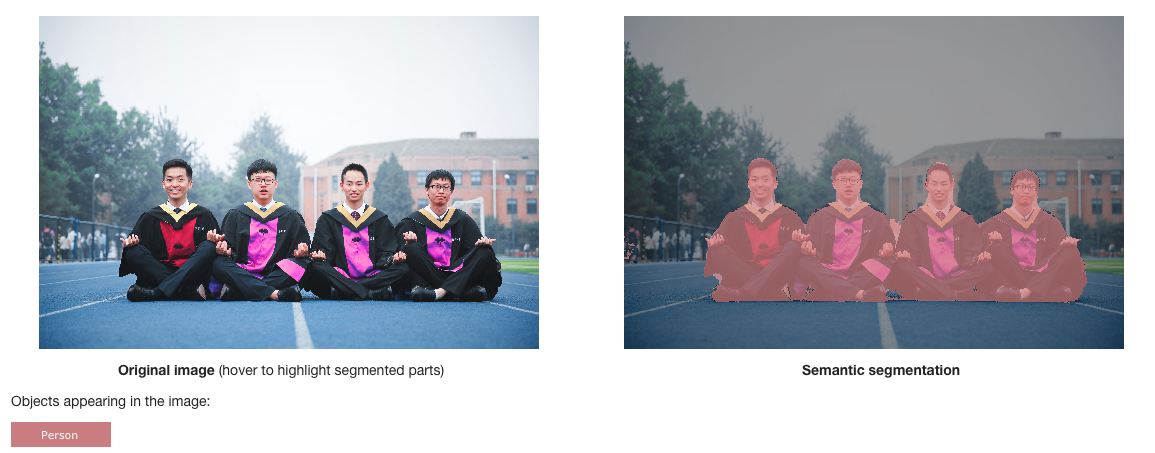
\includegraphics[width=0.9\textwidth]{images/segdemo.png}
	\caption{\label{demo}使用CRF as RNN\upcite{zheng2015conditional}进行图像分割的示例}
\end{figure}
\end{frame}
\section{评价指标}
\subsection*{}
\begin{frame}{评价指标}
在图像分割算法中,主要有如下4个评价指标:
\begin{itemize}
	\item pixel accuracy (Acc): 像素准确率
	\item mean pixel accuracy of different categories (mAcc): 类平均像素准确率
	\item mean Intersection-over-Union of different categories (mIoU): 类平均识别准确度
	\item frequency-weighted IoU (fwIoU): 频率加权的识别准确度
\end{itemize}
\end{frame}

\begin{frame}{IoU示意图}
IoU识别准确度示意图如图\ref{IoU}所示
\begin{figure}
	\centering
	\begin{minipage}[t]{0.45\textwidth}
		\centering
		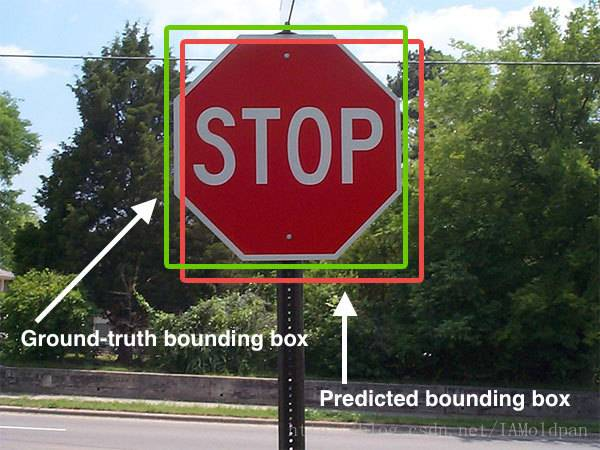
\includegraphics[width=4cm]{images/IoU1.jpg}
	\end{minipage}
	\begin{minipage}[t]{0.45\textwidth}
		\centering
		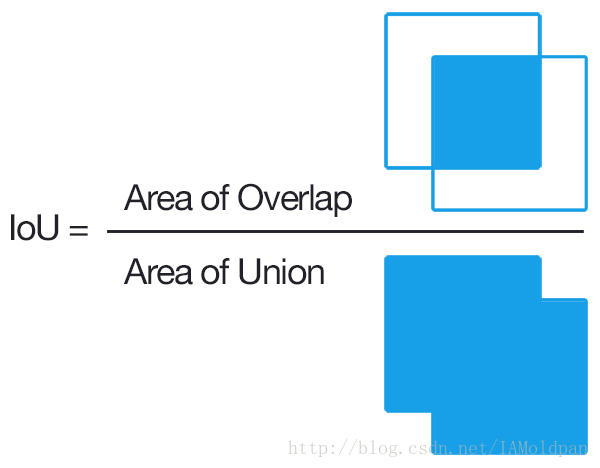
\includegraphics[width=4cm]{images/IoU2.png}
	\end{minipage}
	\caption{\label{IoU}IoU表示含义示意图}
\end{figure}
\end{frame}

\begin{frame}{评价指标的计算方式}
四个指标的计算方式如式\ref{eval}所示:
\begin{block}{定义}
	\begin{equation}
	\label{eval}
	\begin{aligned}
	Acc &= \sum_{i}\frac{n_{ii}}{s} \\
	mAcc &= \frac{1}{n_C}\sum_{i}\frac{n_{ii}}{s_i} \\
	mIoU &= \frac{1}{n_C}\sum_{i}\frac{n_{ii}}{s_i+\sum_{j}n_{ji}-n_{ii}} \\
	fwIoU &= \frac{1}{s}\sum_{i}s_i\frac{n_{ii}}{s_i+\sum_{j}n_{ji}-n_{ii}}
	\end{aligned}
	\end{equation}
\end{block}
\end{frame}



\section{相关算法}

\subsection{FCN}
\begin{frame}{Fully Convolutional Networks}
文章Fully convolutional networks for semantic segmentation\upcite{long2015fully}是2015年CVPR的best paper,在这篇文章中首次提出了全卷积网络。

主要涉及以下3个技术:
\begin{itemize}
	\item 卷积化(Convolutionalization);
	\item 上采样(Upsampling),也叫反卷积(Deconvoltion);
	\item 跳跃结构(Skip Architecture)
\end{itemize}
\end{frame}

\begin{frame}{卷积化}
\qquad 即将传统CNN网络中的全连接层全都转换为卷积层。如图\ref{fcn}所示,上图为AlexNet网络结构,将其中第6、7、8的全连接层全部转换为$1\times1$的卷积层,生成全卷积网络结构。
\begin{figure}
	\centering
	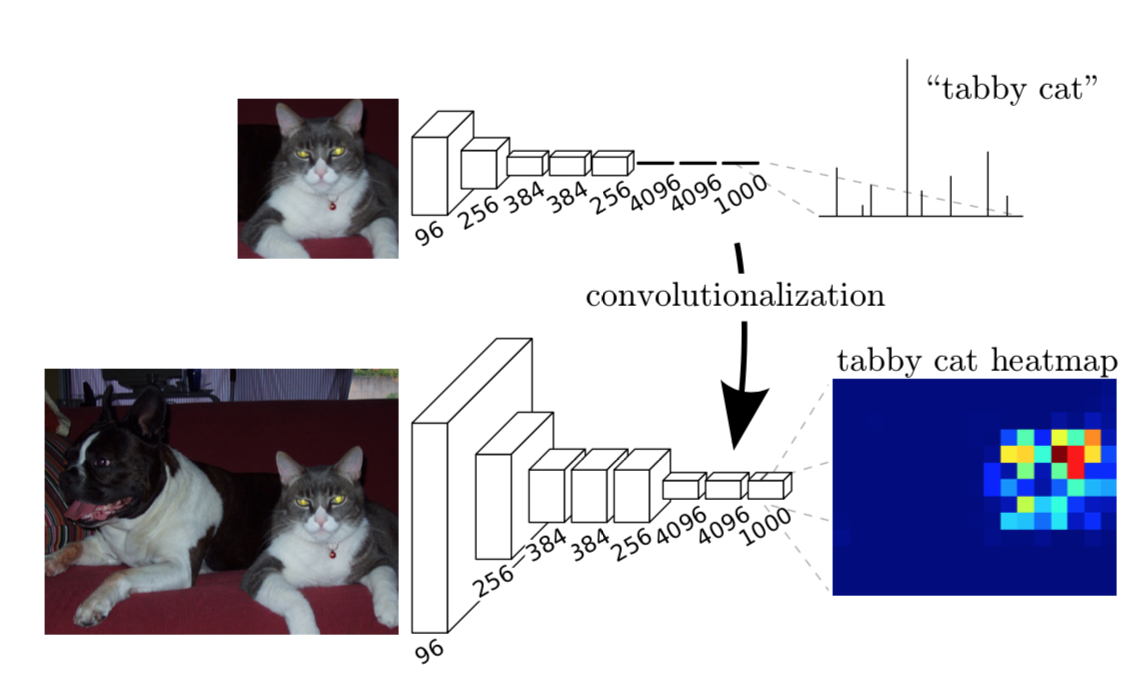
\includegraphics[width=0.7\textwidth]{images/fcn.png}
	\caption{\label{fcn}全卷积网络示例}
\end{figure}
\end{frame}
\begin{frame}{上采样(反卷积)}
由于经过全卷积网络之后得到的feature map相比于原图像要小,为了得到跟原图像一样的feature map,FCN采用上采样的方式将最后一层的feature map放大,得到图\ref{fcn}中的heatmap。

\begin{figure}
	\centering
	\begin{minipage}[t]{0.45\textwidth}
		\centering
		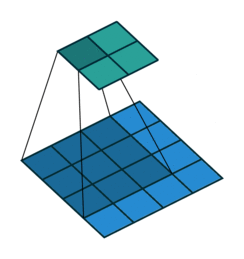
\includegraphics[width=3cm]{images/no_padding_no_strides-0.png}
		\caption{\label{conv}卷积运算示意图}
	\end{minipage}
	\begin{minipage}[t]{0.45\textwidth}
		\centering
		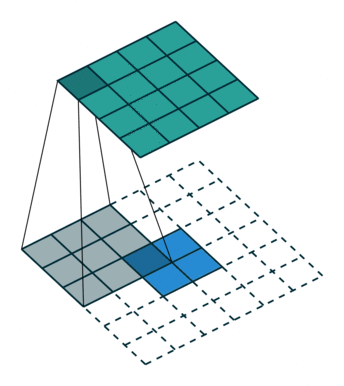
\includegraphics[width=3cm]{images/no_padding_no_strides_transposed-0.png}
		\caption{\label{deconv}反卷积运算示意图\upcite{dumoulin2016guide}}
	\end{minipage}
	
\end{figure}
\end{frame}

\begin{frame}{跳跃结构}
\qquad 在浅层处减小upsampling的步长,得到的fine layer 和 高层得到的coarse layer做融合,然后再upsampling得到输出。使用这样的跳跃结构可以使得分割图中边缘部分较好。如图\ref{skip}所示

\begin{figure}[h]
	\centering
	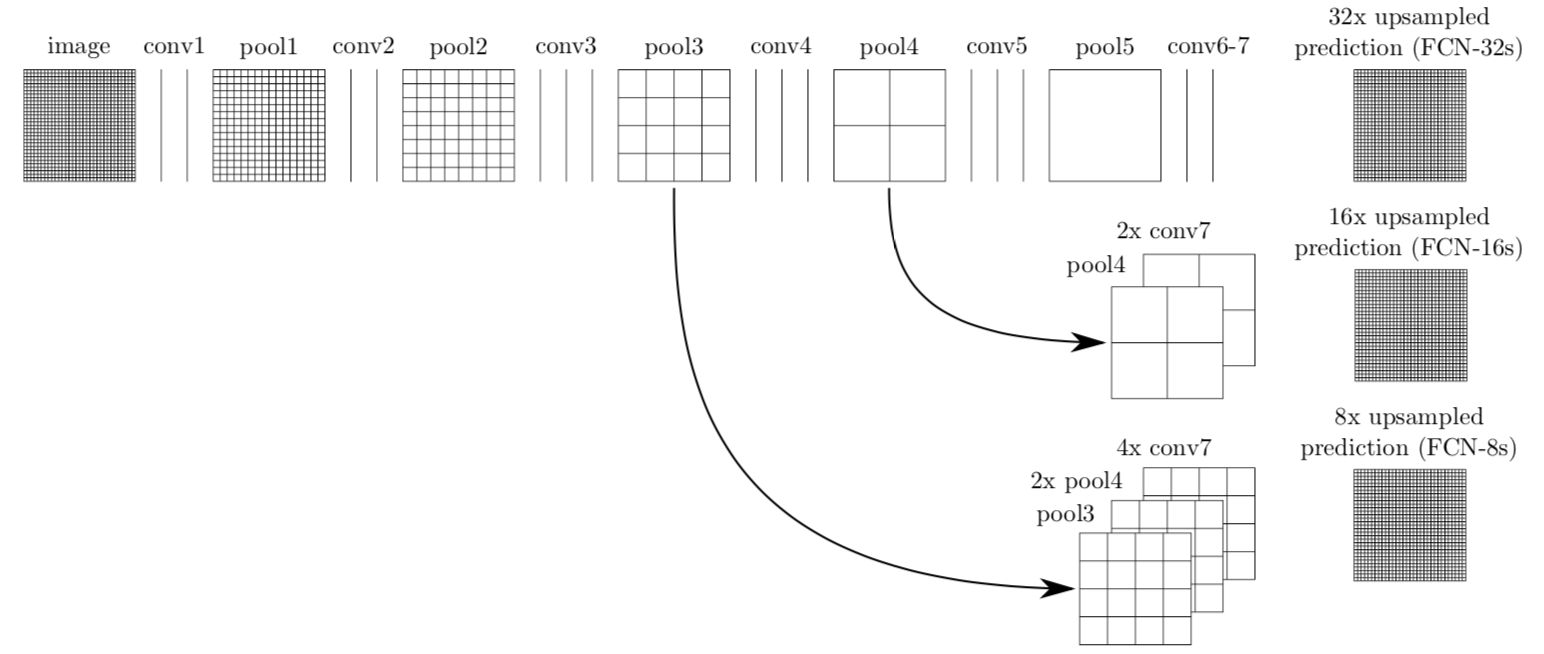
\includegraphics[width=0.8\textwidth]{images/skip.png}
	\caption{\label{skip}跳跃结构示意图}
\end{figure}
\end{frame}

\subsection{DeepLabV1 \& DeepLabV2}
\begin{frame}{DeepLabV1 \& DeepLabV2}
虽然FCN的出现已经比之前传统的CNN的分割效果好了很多,但是还是比较粗糙,细节不太明显,DeepLabV1\upcite{chen2014semantic}和DeepLabV2\upcite{chen2018deeplab}在FCN的基础上采用以下两点改进使得分割效果得到提升。
\begin{itemize}
	\item 空洞卷积(Atrous, Dilated Conv);
	\item 条件随机场(CRF)
\end{itemize}

\begin{figure}[h]
	\centering
	\begin{minipage}[t]{0.4\textwidth}
		\centering
		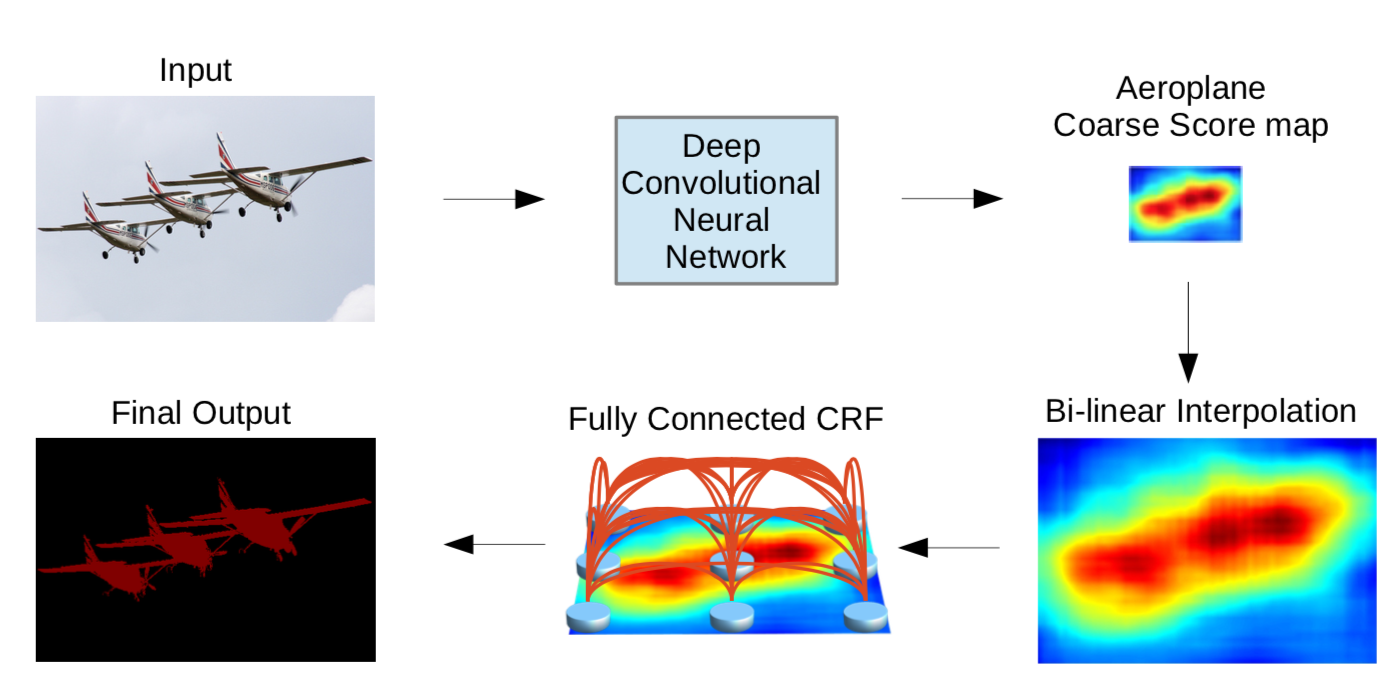
\includegraphics[width=4.5cm]{images/deeplabv1.png}
		\caption{\label{deeplabv1}DeepLabV1示意图}
	\end{minipage}
	\begin{minipage}[t]{0.4\textwidth}
		\centering
		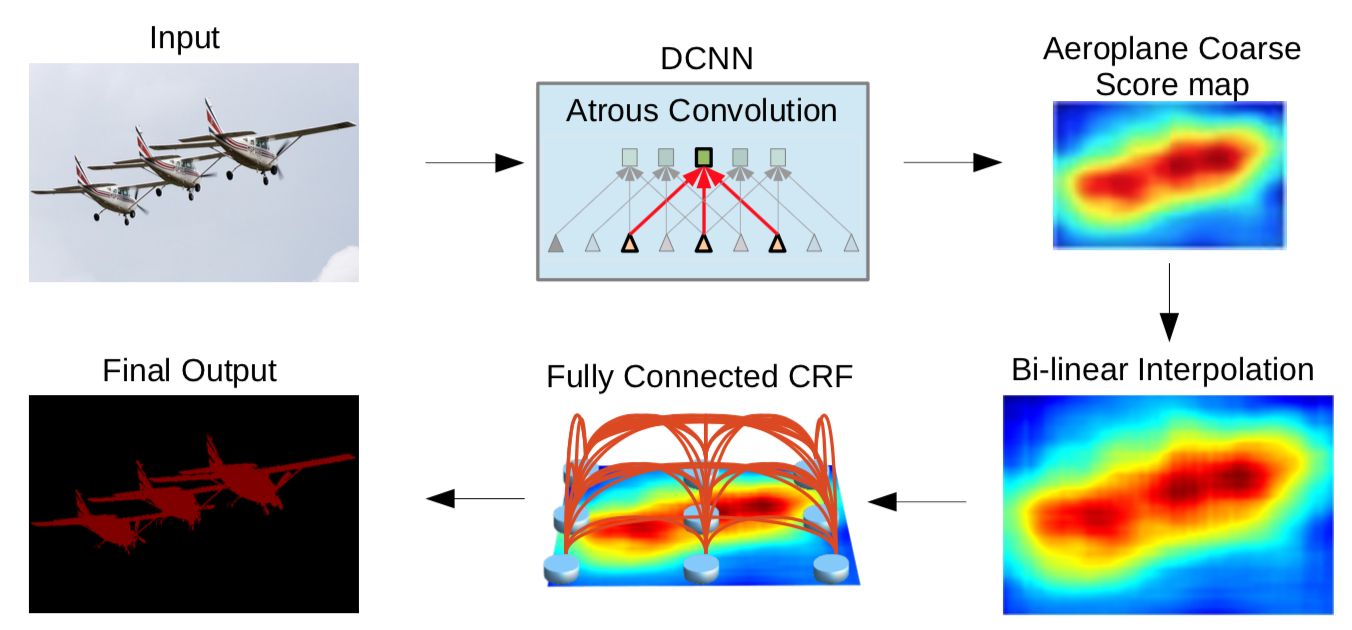
\includegraphics[width=4.5cm]{images/deeplabv2.png}
		\caption{\label{deeplabv2}DeepLabV2示意图}
	\end{minipage}
\end{figure}
\end{frame}

\begin{frame}{空洞卷积}
	空洞卷积(Dilate Conv)首次出现于论文\cite{yu2015multi}中。由于普通的卷积感受野较小,需要增加池化层来增加感受野,但是池化层又会损失信息,所以提出空洞卷积来在不损失信息的情况下增加感受野的范围。如图\ref{dilate}所示
	
	\begin{figure}[h]
		\centering
		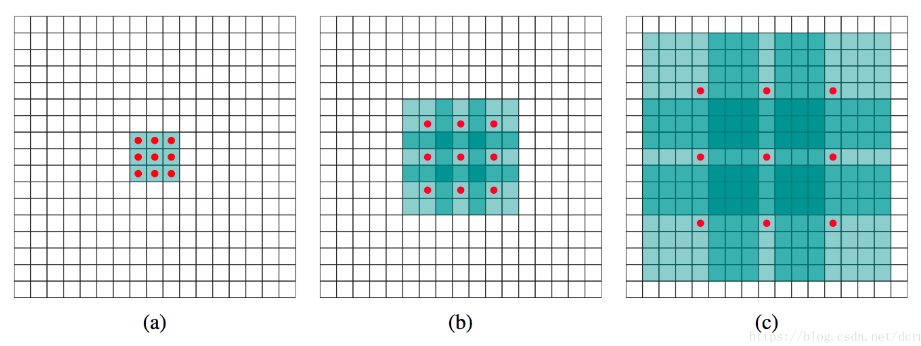
\includegraphics[width=0.7\textwidth]{images/dilateconv.png}
		\caption{\label{dilate}空洞卷积示意图.(a)表示普通的卷积,卷积核为$3\times 3$,感受野也为$3\times 3$,较小;(b)表示扩张系数为2的空洞卷积,卷积核为$3\times 3$,但是感受野有$7\times 7$,比之前大了一点;(c)表示扩张系数为4的空洞卷积,卷积核为$3\times 3$,但是感受野有$15\times 15$,更大了}
	\end{figure}
\end{frame}



\begin{frame}{条件随机场}
只用DCNN能够预测到目标的大概位置但是比较模糊,论文\cite{krahenbuhl2011efficient}中提出的全连接条件随机场尝试找到图像像素之间的关系:相近且相似的像素大概率为同一标签,考虑像素的概率分配标签,迭代细化结果。如图\ref{crf}所示。

\begin{figure}[h]
	\centering
	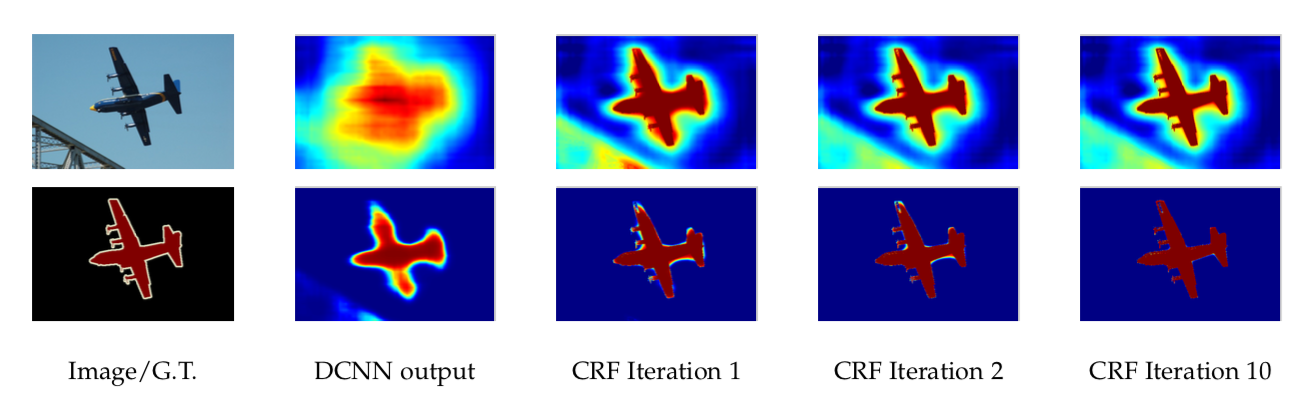
\includegraphics[width=0.9\textwidth]{images/crf.png}
	\caption{\label{crf}使用CRF细化分割效果。可以看出,随着迭代次数的增加,图像分割的效果逐渐增强}
\end{figure}
\end{frame}

\begin{frame}{DeepLabV1网络结构}
如图\ref{vgg16}和\ref{vgg16dial},DeepLabV1网络是在VGG16网络结构的基础上进行了如下修改:
\begin{itemize}
	\item 全连接层转为卷积层;
	\item 最后的两个池化层去掉下采样;
	\item 后续的卷积层转为空洞卷积;
	\item 使用ImageNet上预训练的参数进行finetune。
\end{itemize}

\begin{figure}[h]
	\centering
	\begin{minipage}[t]{0.4\textwidth}
		\centering
		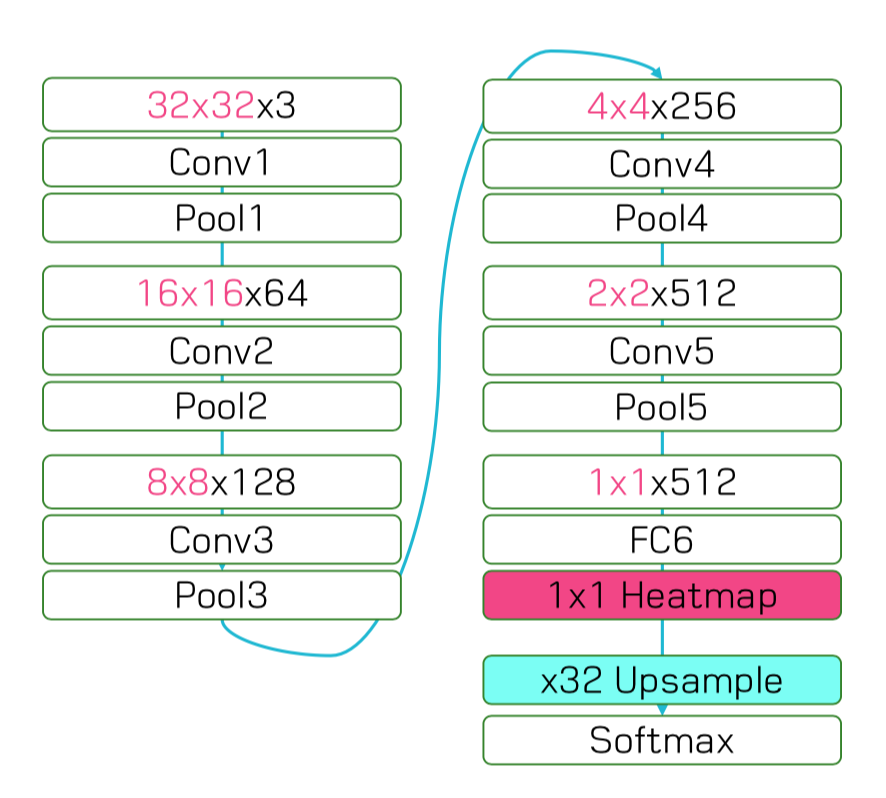
\includegraphics[width=3cm]{images/vgg16.png}
		\captionsetup{font={scriptsize}}
		\caption{\label{vgg16}VGG16网络结构示例}
	\end{minipage}
	\begin{minipage}[t]{0.4\textwidth}
		\centering
		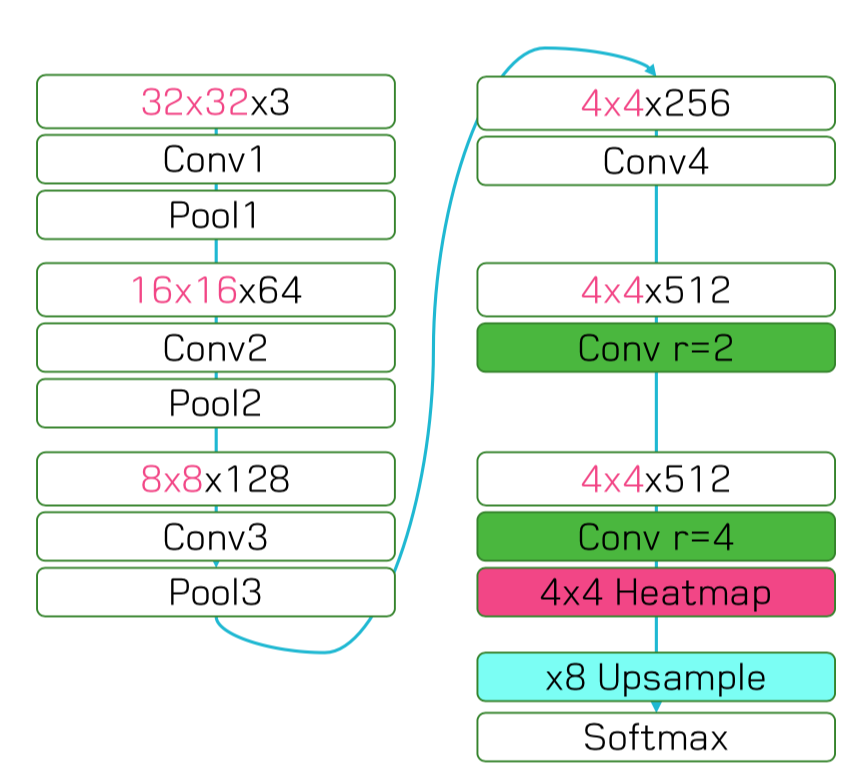
\includegraphics[width=3cm]{images/vgg16dial.png}
		\captionsetup{font={scriptsize}}
		\caption{\label{vgg16dial}VGG16网络修改后的DeepLabV1网络结构示例}
	\end{minipage}
\end{figure}

\end{frame}

\begin{frame}{ASPP模块}
DeepLabV2相对于DeepLabV1使用了ASPP(Atrous Spatial Pyramid Pooling)模块获得了更好的分割效果。ASPP在给定的Input Feature Map上以不同的扩充率做空洞卷积并进行采样,最后将结果融合起来作为输出。

\begin{figure}[h]
	\centering
	\begin{minipage}[t]{0.4\textwidth}
		\centering
		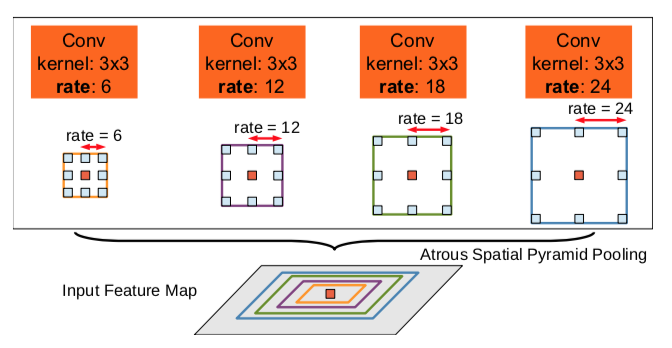
\includegraphics[width=4cm]{images/aspp1.png}
		\caption{\label{aspp1}ASPP模块示意图}
	\end{minipage}
	\begin{minipage}[t]{0.4\textwidth}
		\centering
		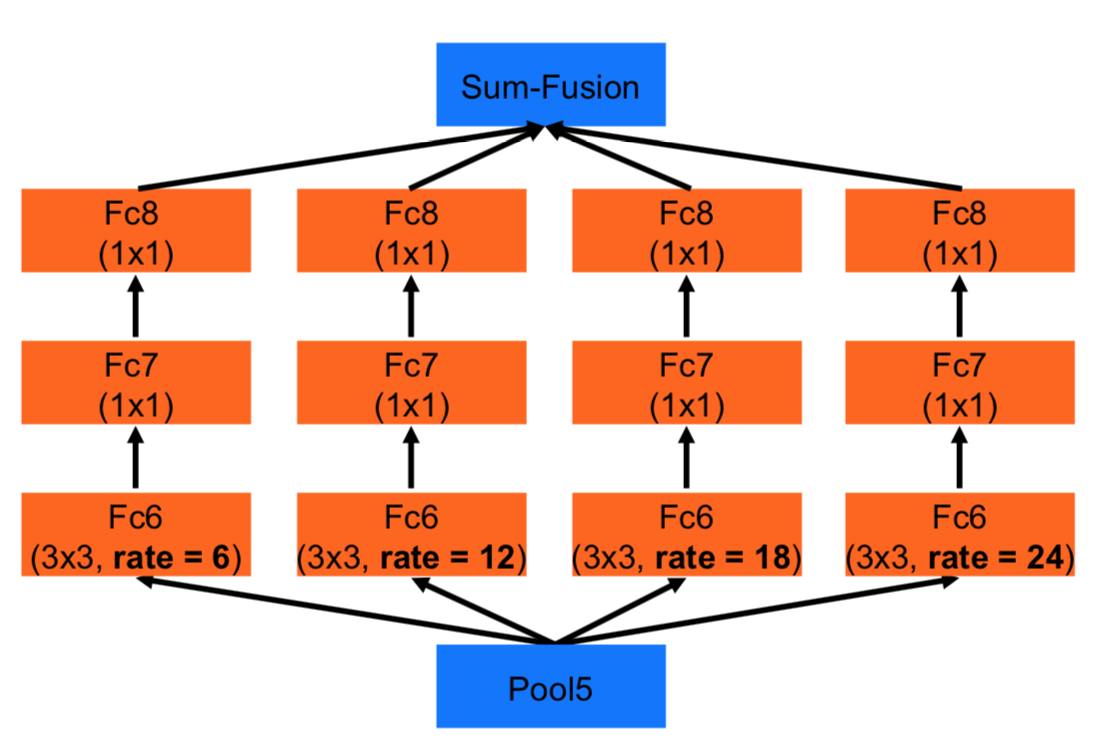
\includegraphics[width=4cm]{images/aspp2.png}
		\caption{\label{aspp2}ASPP结构示意图}
	\end{minipage}
\end{figure}

\end{frame}

\begin{frame}{DeepLabV1 $\to$ DeepLabV2}
\begin{itemize}
	\item 基础网络结构由VGG16转为ResNet;
	\item 使用了ASPP模块;
	\item 使用了不同的学习策略
	\item 使用MS-COCO数据集上预训练的参数进行finetune
\end{itemize}

\begin{figure}[h]
	\centering
	\begin{minipage}[t]{0.4\textwidth}
		\centering
		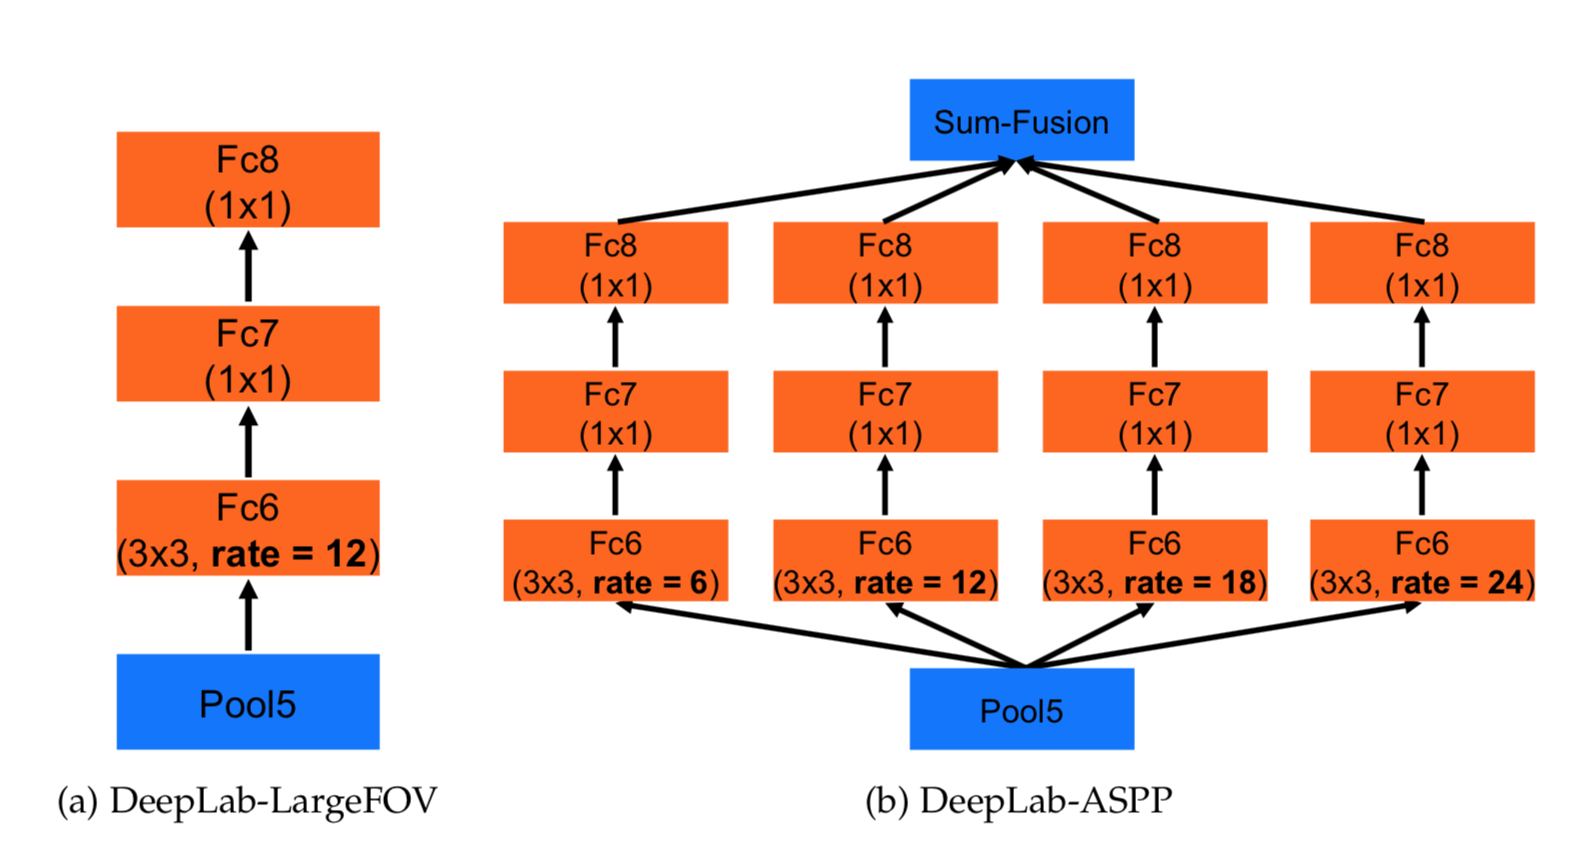
\includegraphics[width=4.5cm]{images/v1vsv2.png}
		\caption{\label{v1vsv2}结构对比图}
	\end{minipage}
	\begin{minipage}[t]{0.4\textwidth}
		\centering
		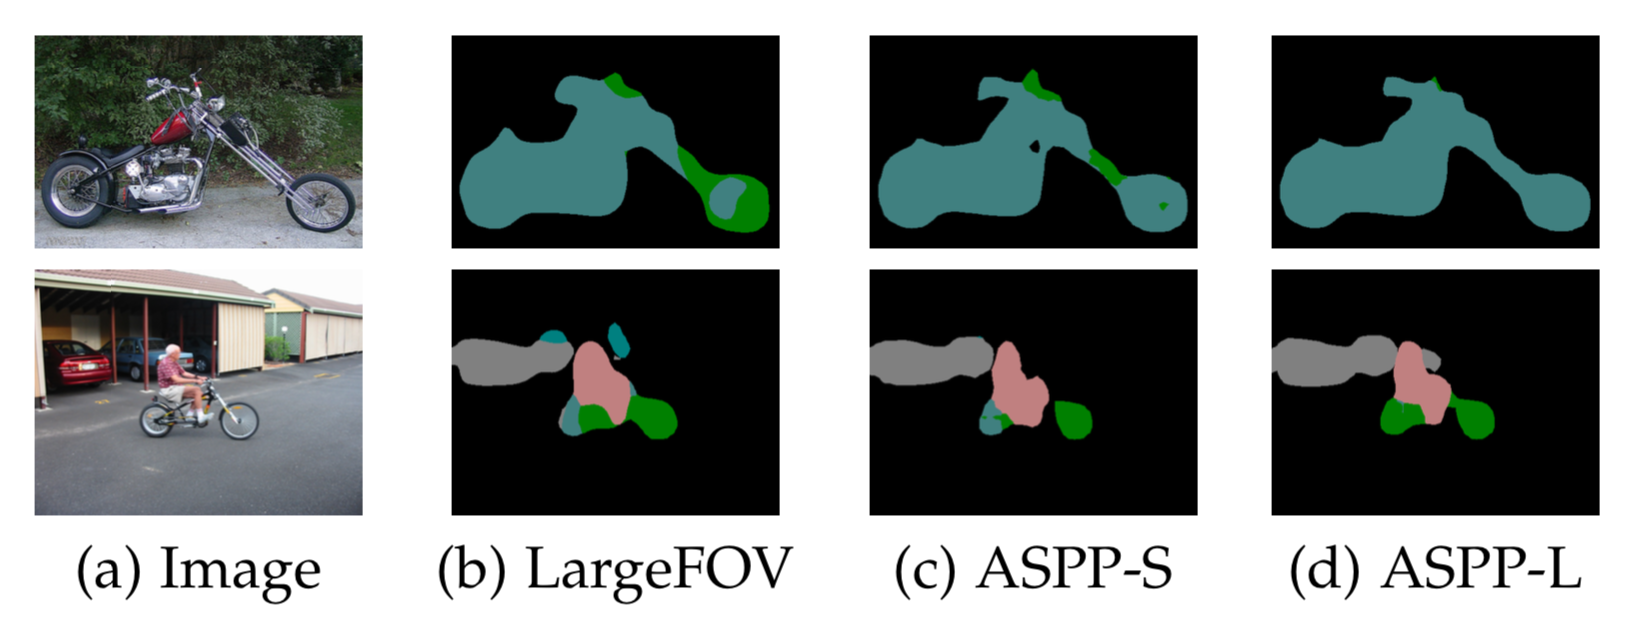
\includegraphics[width=4.5cm]{images/v1vsv2res.png}
		\caption{\label{v1vsv2res}结果对比图}
	\end{minipage}
\end{figure}
\end{frame}

\subsection{DeepLabV3}
\begin{frame}{DeepLabV3}
\only<1>{
DeepLab系列的第三篇文章\upcite{chen2017rethinking},相比于V1和V2有如下变化:
\begin{itemize}
	\item 提出了更通用的框架,适用于任何网络;
	\item 复制了ResNet最后的block并且级联起来;
	\item 在ASPP中使用BN层,并且有新的ASPP结构;
	\item 没有使用CRF。
\end{itemize}
}
\only<2>{
	如图\ref{deeplabv3}所示。复制ResNet最后一个block的多个副本,并且级联起来,图\ref{deeplabv3}中的block5-7是block4的副本。每个block中包含三个卷积(MultiGrid),每个block中最后一个卷积的步长为2(最后一个block除外),为了维持原图尺寸,使用不同采样率的空洞卷积来代替原来的卷积。
}

\begin{figure}[h]
	\centering
	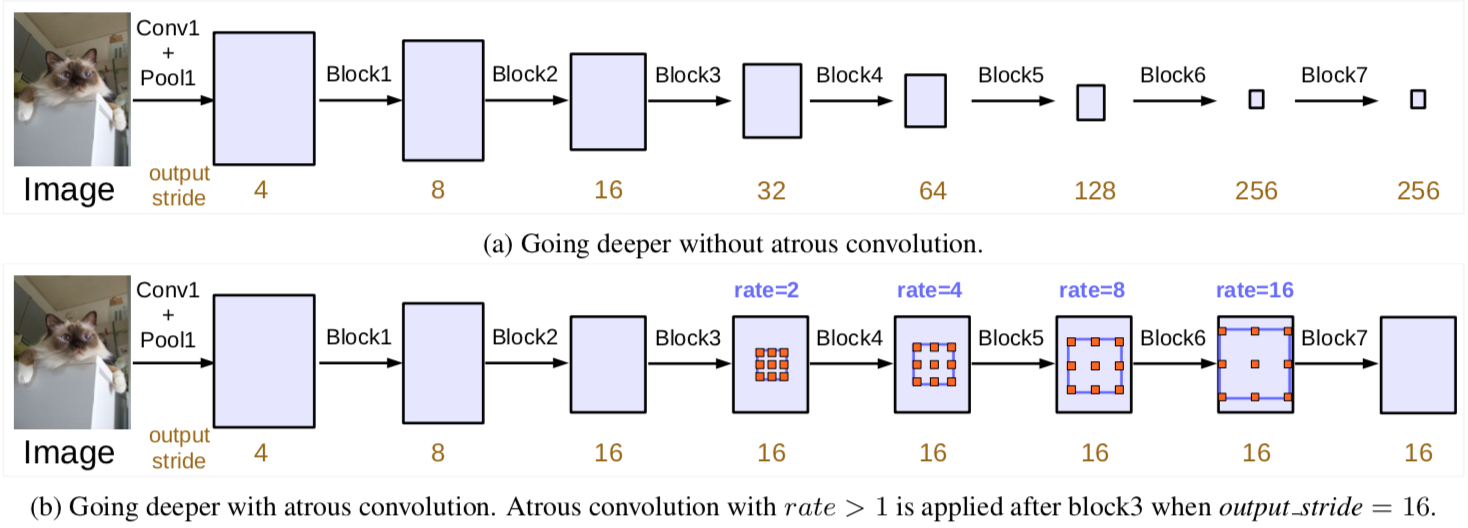
\includegraphics[width=0.8\textwidth]{images/deeplabv3.png}
	\caption{\label{deeplabv3}级联模块使用空洞卷积和不使用空洞卷积的示意图}
\end{figure}
\end{frame}

%\begin{frame}{网络结构}
%
%如图\ref{deeplabv3}所示。复制ResNet最后一个block的多个副本,并且级联起来,图\ref{deeplabv3}中的block5-7是block4的副本。每个block中包含三个卷积(MultiGrid),每个block中最后一个卷积的步长为2(最后一个block除外),为了维持原图尺寸,使用不同采样率的空洞卷积来代替原来的卷积。
%\begin{figure}[h]
%	\centering
%	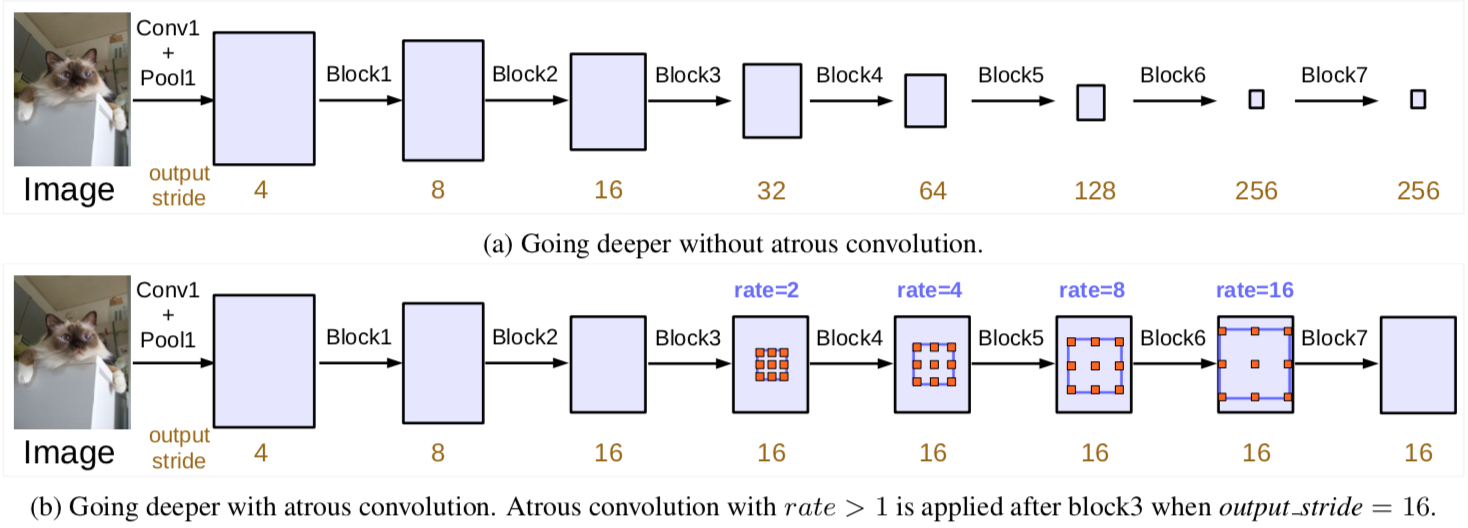
\includegraphics[width=0.8\textwidth]{images/deeplabv3.png}
%	\caption{\label{deeplabv3}级联模块使用空洞卷积和不使用空洞卷积的示意图}
%\end{figure}
%\end{frame}

\begin{frame}{新的ASPP模块}
相比于原ASPP模块有如下改变:
\begin{itemize}
	\item ASPP中应用了BN层;
	\item 随着采样率的增加,卷积核中有效的权重减小了;
	\item 使用模型最后的feature map做全局平均池化;
	\item 包括一个$1\times 1$的卷积和3个$3\times 3$采样率分别为(6,12,18)的空洞卷积,并且每个卷积都有BN层和一个全局平均池化层;
	\item 所有的分支通过$1\times 1$的卷积级联起来。
\end{itemize}

\begin{figure}[h]
	\centering
	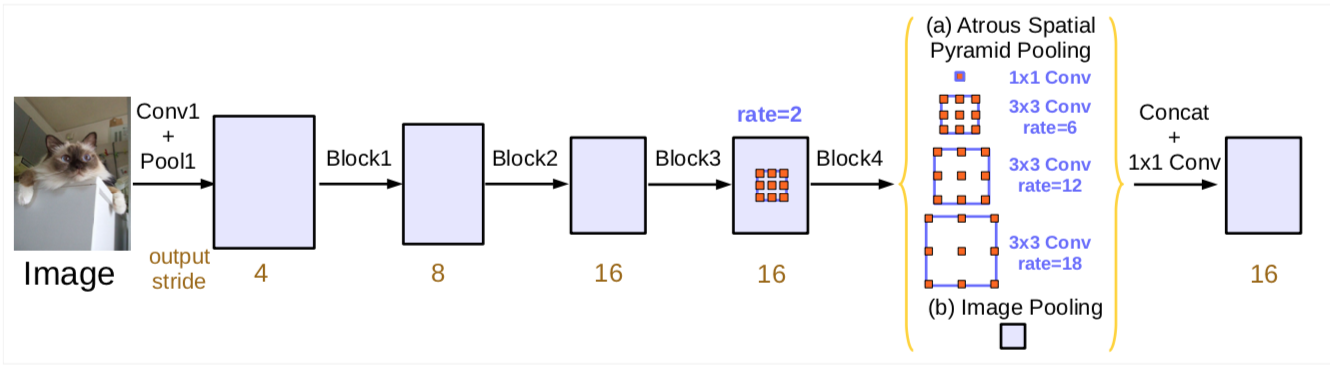
\includegraphics[width=0.8\textwidth]{images/asppnew.png}
	\caption{\label{asppnew}新的ASPP模块}
\end{figure}

\end{frame}

\begin{frame}{实验结果对比}
以上算法在PASCAL VOC 2012 \upcite{everingham2015pascal}上的实验结果对比如图\ref{result0}所示:
\begin{figure}[h]
	\centering
	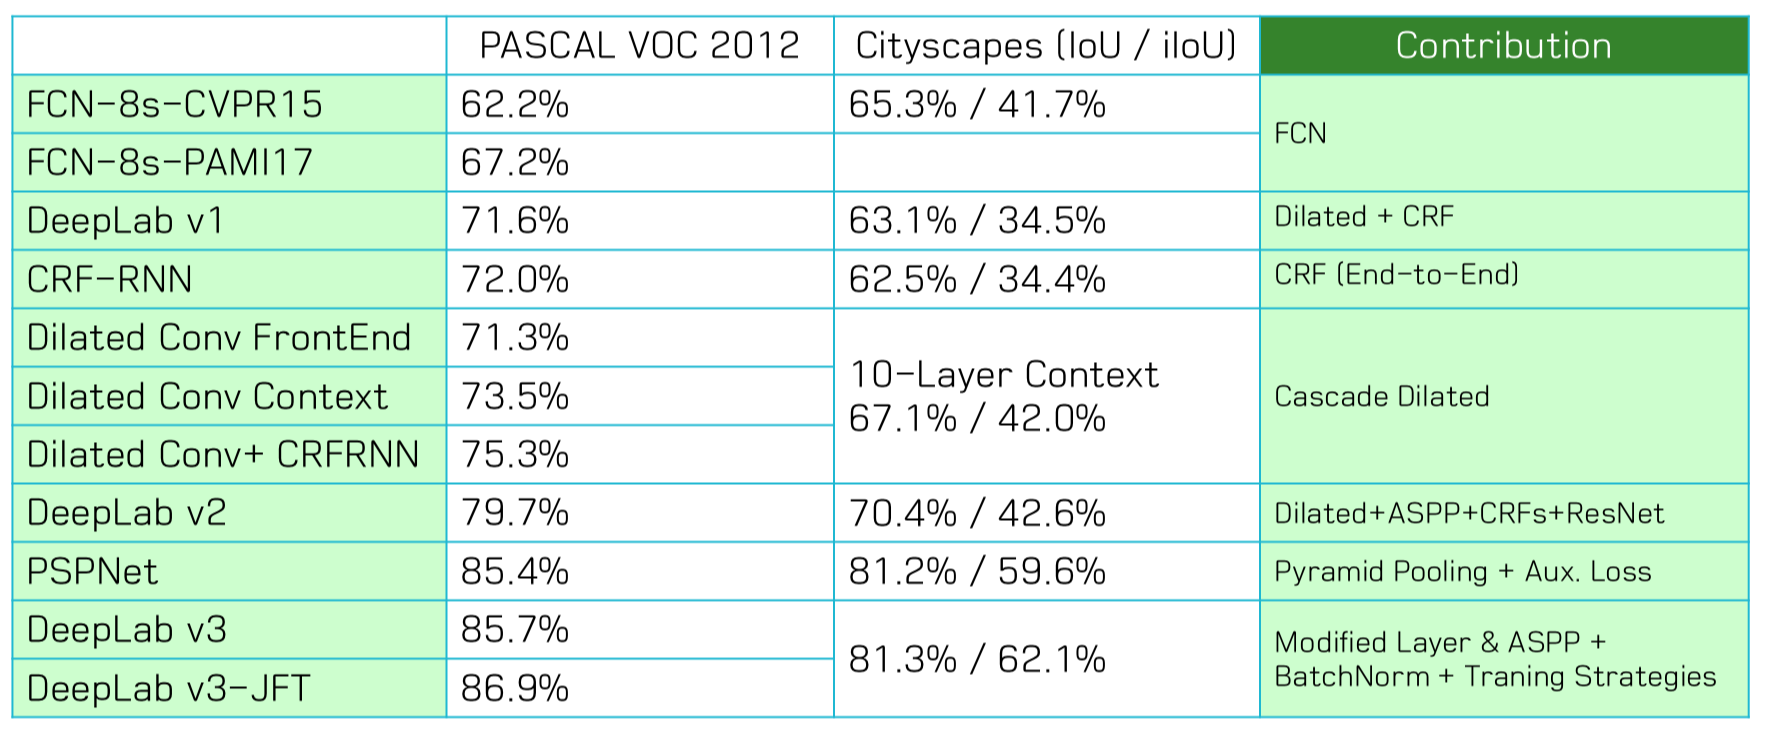
\includegraphics[width=0.9\textwidth]{images/result0.png}
	\caption{\label{result0}PASCAL VOC 2012实验结果对比}
\end{figure}
\end{frame}

\subsection{Depth-aware CNN}
\begin{frame}{Depth-aware CNN Introduction}
\href{http://openaccess.thecvf.com/content_ECCV_2018/papers/Weiyue_Wang_Depth-aware_CNN_for_ECCV_2018_paper.pdf}{文章Depth-aware CNN for RGB-D Segmentation}\upcite{wang2018depth} 是ECCV 2018上关于图像语义分割的一篇论文,针对RGB-D的图像提出了一种新的算法。

此前关于RGB-D图像的分割方法主要有:
\begin{itemize}
	\item 使用全卷积网络FCN将RGB信息和Depth信息使用两个独立的CNN来进行处理。这样处理会使得参数量和训练时间变为单个CNN的两倍,并且像素之间的关联也因此变弱。
	\item 使用3D networks来处理深度信息,但是这样操作会使得计算复杂度提升很多。
\end{itemize}
这篇论文提出了一种使用2D CNN来处理RGB-D图像语义分割的算法。
\end{frame}

\begin{frame}{Depth-aware CNN Introduction}
为了解决像素之间深度信息关联性以及计算复杂度,参数量过多的问题,算法主要采用以下3个方式来解决:
\begin{itemize}
	\item 2D CNN。使用传统的2D卷积神经网络结构不引入新的变量可以解决参数量过多、计算量过大的问题;
	\item depth-aware convolution。定义一种新的卷积方式来处理像素间深度信息关联问题;
	\item depth-aware average pooling。类似于depth-aware convolution,定义一种新的均值池化方式来处理像素间关联的问题。
\end{itemize}
\end{frame}

\begin{frame}{Depth-aware Convolution}
\begin{figure}[h]
	\centering
	\begin{minipage}[t]{0.4\textwidth}
		\centering
		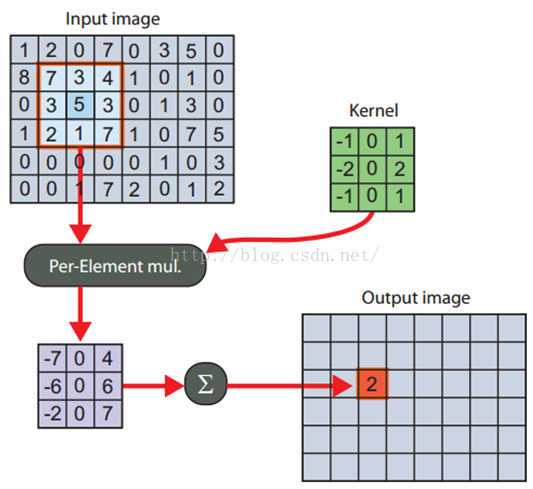
\includegraphics[width=4cm]{images/sconv.png}
		\caption{\label{sconv}传统的卷积操作}
	\end{minipage}
	\begin{minipage}[t]{0.4\textwidth}
		\centering
		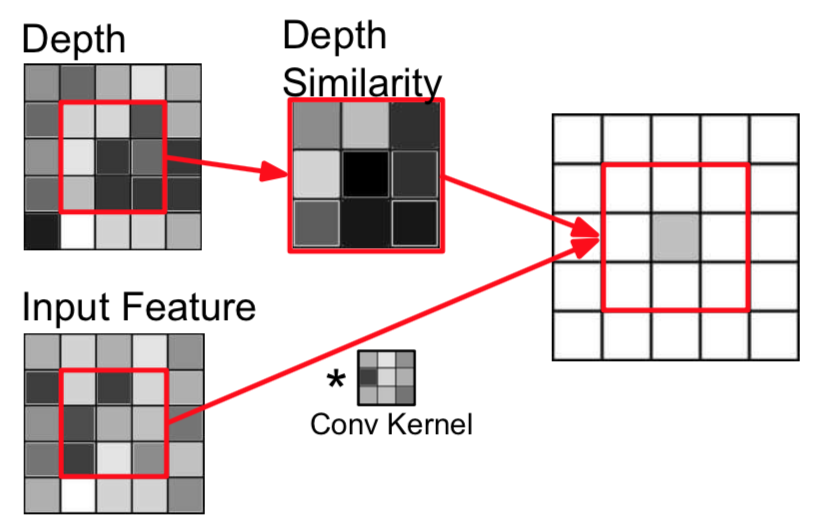
\includegraphics[width=4cm]{images/dconv.png}
		\caption{\label{dconv}depth-aware卷积操作}
	\end{minipage}
\end{figure}
\end{frame}

\begin{frame}[<+->]{Depth-aware Convolution}

\begin{block}{standard 2D convolution}
	\begin{equation}
	\mathrm{y}(\mathrm{p}_0)=\sum_{\mathrm{p}_n\in \mathcal{R}}\mathrm{w}(\mathrm{p}_n)\cdot \mathrm{x}(\mathrm{p}_0+\mathrm{p}_n)
	\end{equation}
	如图\ref{sconv}所示。其中 $\mathcal{R}$是$\mathrm{p}_0$的邻域,$\mathrm{w}$是卷积核。
\end{block}

\begin{block}{depth-aware convolution}
	\begin{equation}
	\label{dconv:eq}
	\mathrm{y}(\mathrm{p}_0)=\sum_{\mathrm{p}_n\in \mathcal{R}}\mathrm{w}(\mathrm{p}_n)\cdot \mathrm{F_D}(\mathrm{p}_0,\mathrm{p}_0+\mathrm{p}_n)\cdot\mathrm{x}(\mathrm{p}_0+\mathrm{p}_n)
	\end{equation}
	如图\ref{dconv}所示。其中$\mathrm{F_D}$表示像素之间深度信息的关联:
	\begin{equation}
	\label{depthFunction}
	\mathrm{F_D}(\mathrm{p}_i,\mathrm{p}_j)=\exp(-\alpha|\mathrm{D}(\mathrm{p}_i)-\mathrm{D}(\mathrm{p}_j)|)
	\end{equation}
\end{block}
\end{frame}

%\begin{frame}
%\begin{block}{depth-aware convolution}
%	\begin{equation}
%	\label{dconv:eq}
%	\mathrm{y}(\mathrm{p}_0)=\sum_{\mathrm{p}_n\in \mathcal{R}}\mathrm{w}(\mathrm{p}_n)\cdot \mathrm{F_D}(\mathrm{p}_0,\mathrm{p}_0+\mathrm{p}_n)\cdot\mathrm{x}(\mathrm{p}_0+\mathrm{p}_n)
%	\end{equation}
%	如图\ref{dconv}所示。其中$\mathrm{F_D}$表示像素之间深度信息的关联:
%	\begin{equation}
%	\label{depthFunction}
%	\mathrm{F_D}(\mathrm{p}_i,\mathrm{p}_j)=\exp(-\alpha|\mathrm{D}(\mathrm{p}_i)-\mathrm{D}(\mathrm{p}_j)|)
%	\end{equation}
%\end{block}
%\end{frame}


\begin{frame}{Depth-aware Average Pooling}
\begin{figure}[h]
	\centering
	\begin{minipage}[t]{0.4\textwidth}
		\centering
		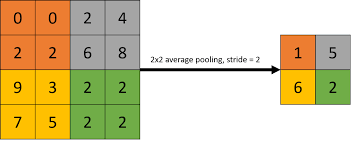
\includegraphics[width=4cm]{images/savg.png}
		\caption{\label{savg}传统的均值池化操作}
	\end{minipage}
	\begin{minipage}[t]{0.4\textwidth}
		\centering
		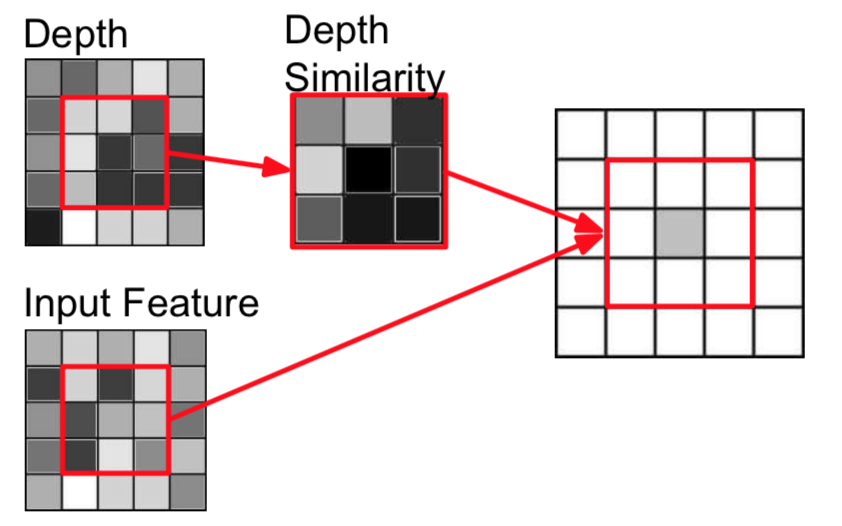
\includegraphics[width=4cm]{images/davg.png}
		\caption{\label{davg}depth-aware均值池化操作}
	\end{minipage}
\end{figure}
\end{frame}

\begin{frame}[<+->]{Depth-aware Average Pooling}

\begin{block}{conventional average pooling}
	\begin{equation}
	\mathrm{y}(\mathrm{p}_0)=\frac{1}{|\mathcal{R}|}\sum_{\mathrm{p}_n\in \mathcal{R}} \mathrm{x}(\mathrm{p}_0+\mathrm{p}_n)
	\end{equation}
	如图\ref{savg}所示。其中 $\mathcal{R}$是$\mathrm{p}_0$的邻域。
\end{block}


\begin{block}{depth-aware average pooling}
	\begin{equation}
	\label{davg:eq}
	\mathrm{y}(\mathrm{p}_0)=\frac{1}{|\mathcal{R}|}\sum_{\mathrm{p}_n\in \mathcal{R}} \mathrm{F_D}(\mathrm{p}_0,\mathrm{p}_0+\mathrm{p}_n)\cdot\mathrm{x}(\mathrm{p}_0+\mathrm{p}_n)
	\end{equation}
	如图\ref{davg}所示。其中$\mathrm{F_D}$如公式\ref{depthFunction}所示表示像素之间深度信息的关联。
\end{block}

\end{frame}

\begin{frame}{网络结构}
本算法使用DeepLab作为baseline,使用了VGG16和ResNet-15的网络结构,将其中的卷积操作改为式\ref{dconv:eq}中的卷积操作,将其中的均值池化操作改为式\ref{davg:eq}中的均值池化操作。网络结构如图\ref{arch}所示。

\begin{figure}[h]
	\centering
	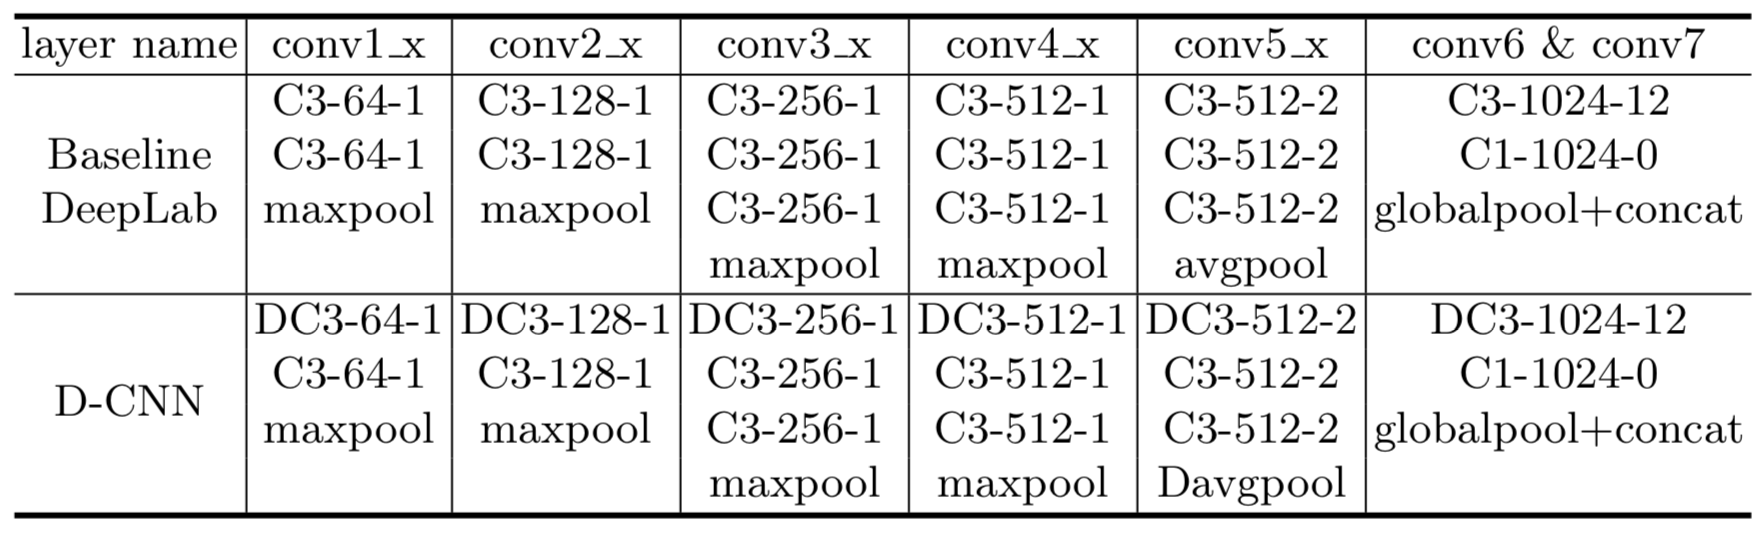
\includegraphics[width=0.9\textwidth]{images/arch.png}
	\caption{\label{arch}DeepLab和DCNN使用VGG16的结构}
\end{figure}
\end{frame}

\begin{frame}[allowframebreaks]{实验结果}
本篇论文将提出的算法与DeepLab的baseline在NYUv2\upcite{silberman2012indoor}数据集上进行测试,NYUv2数据集包括1449像素集标注的RGB-D图像,实验按照40个class,将数据划分为训练集:795张图像和测试集:654张图像进行实验得到如图\ref{res1}和图\ref{res2}所示的结果。

\begin{figure}[h]
	\centering
	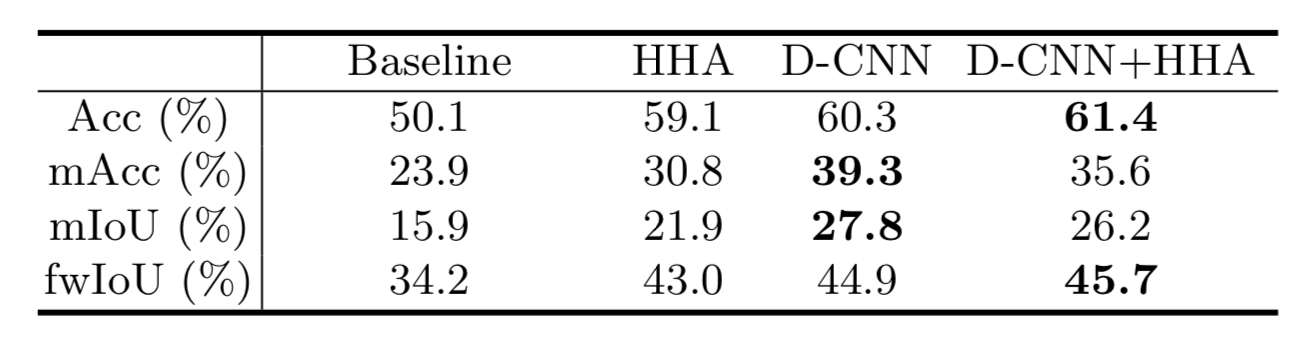
\includegraphics[width=0.9\textwidth]{images/res1.png}
	\caption{\label{res1}DeepLab和DCNN在评价指标上的对比结果}
\end{figure}

\begin{figure}[h]
	\centering
	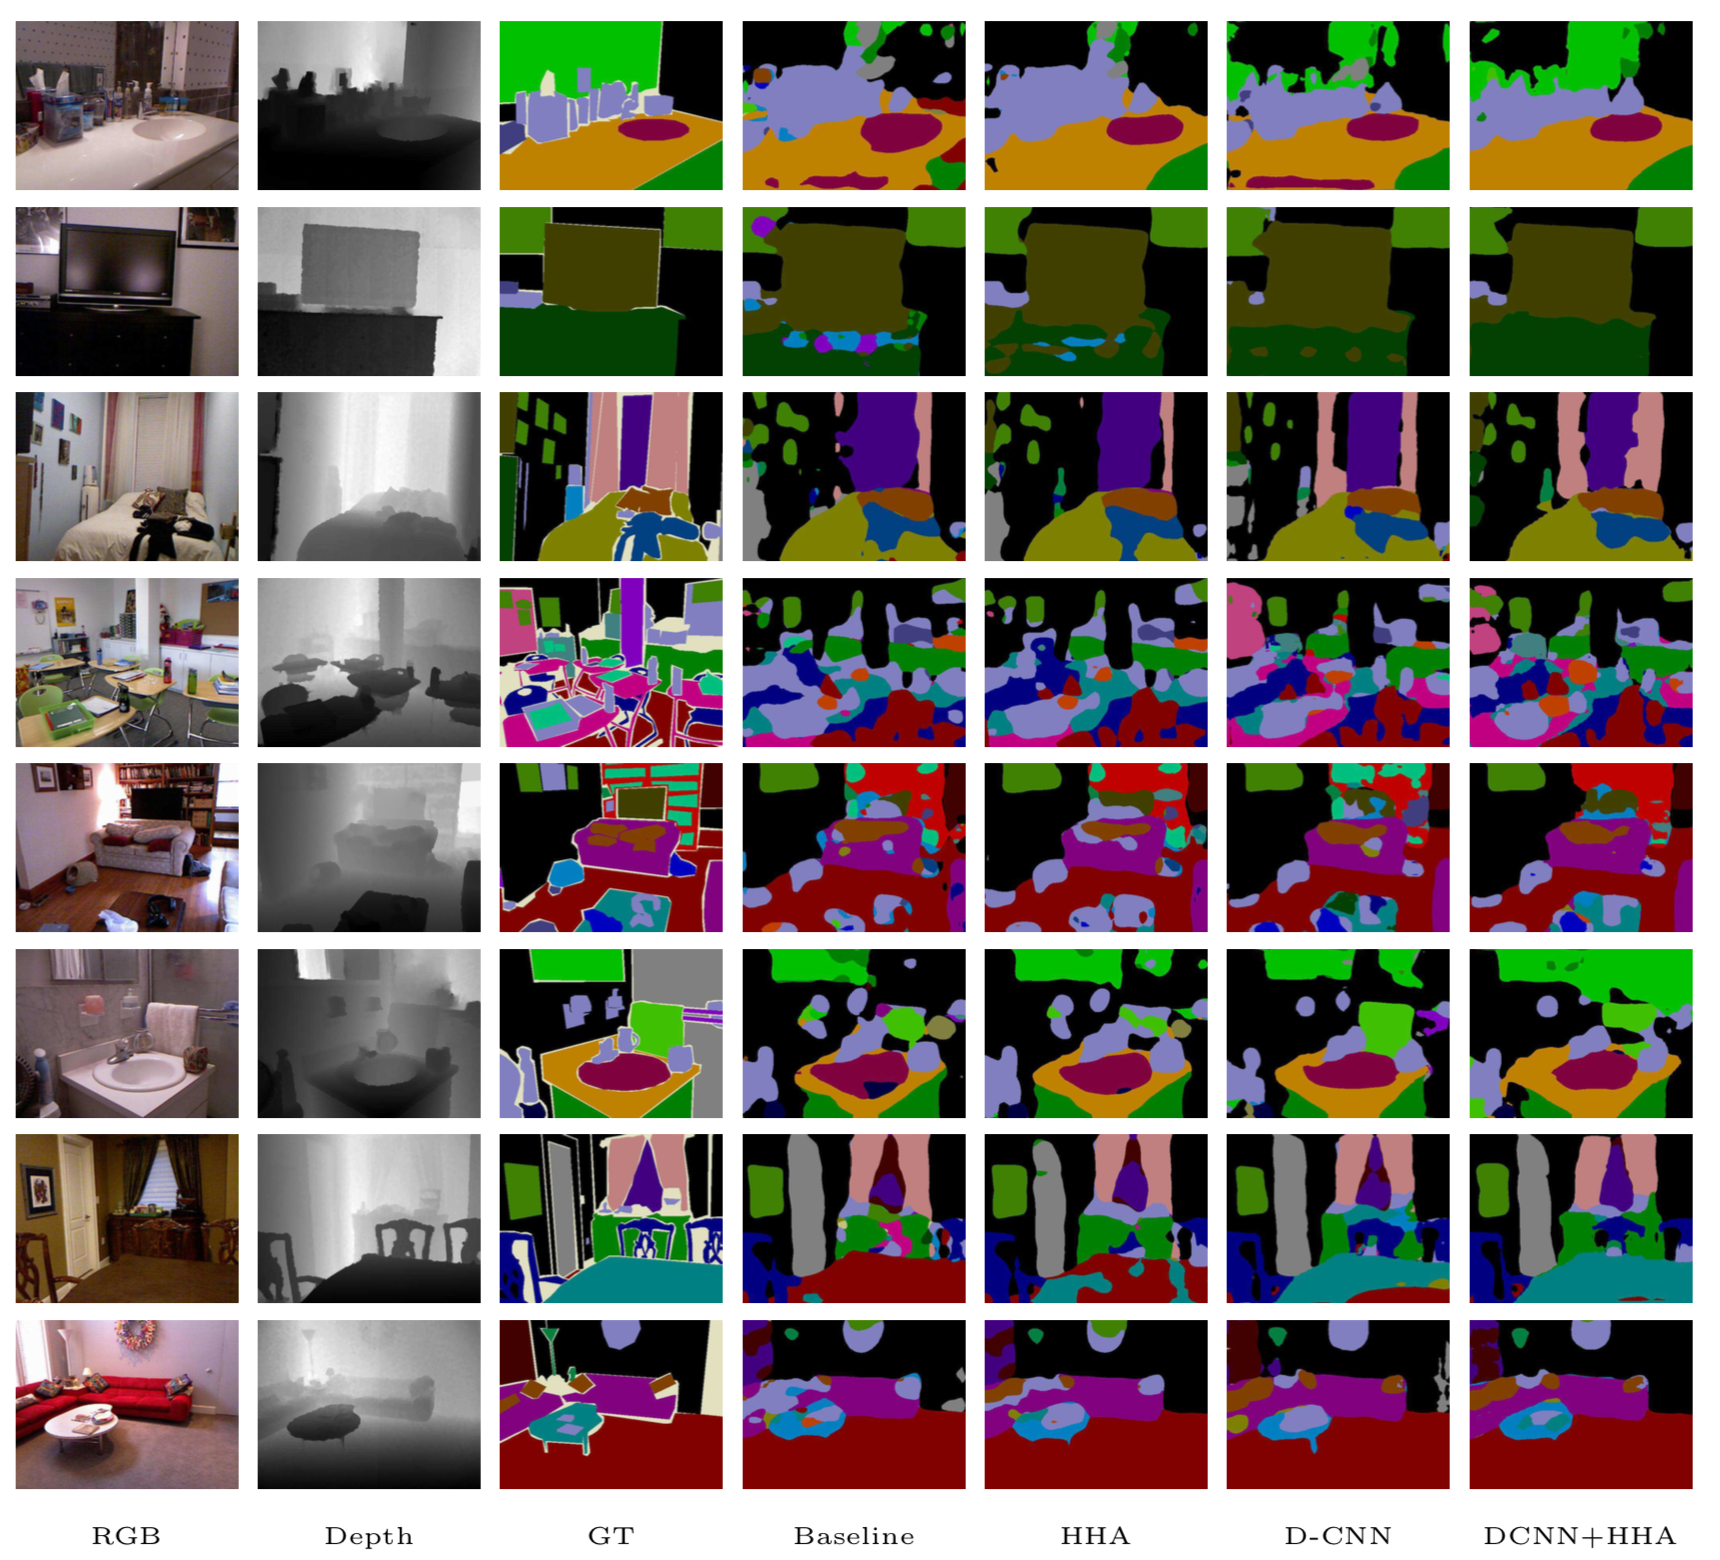
\includegraphics[width=0.65\textwidth]{images/res2.png}
	\caption{\label{res2}DeepLab和DCNN在测试集上的效果图}
\end{figure}
\end{frame}

\begin{frame}[allowframebreaks]{参考文献}
\printbibliography
\end{frame}

%\begin{frame}{THE END}
%\begin{figure}[h]
%	\label{image3}
%	\centering
%	
\includegraphics[height=3cm]{images/thx.jpg}
%\end{figure}
%\end{frame}
\end{document}

%\begin{figure}[h]
%	\label{image1}
%	\centering
%	\includegraphics[height=4cm]{triangle1.jpeg}
%\end{figure}